\section{Ergebnis der UX-Methode des Question Board, das von Dryads Cloud-Team mit dem Miro-Tool erstellt wurde} \label{appendix:question_board}

\begin{figure}[H]
  \centering
  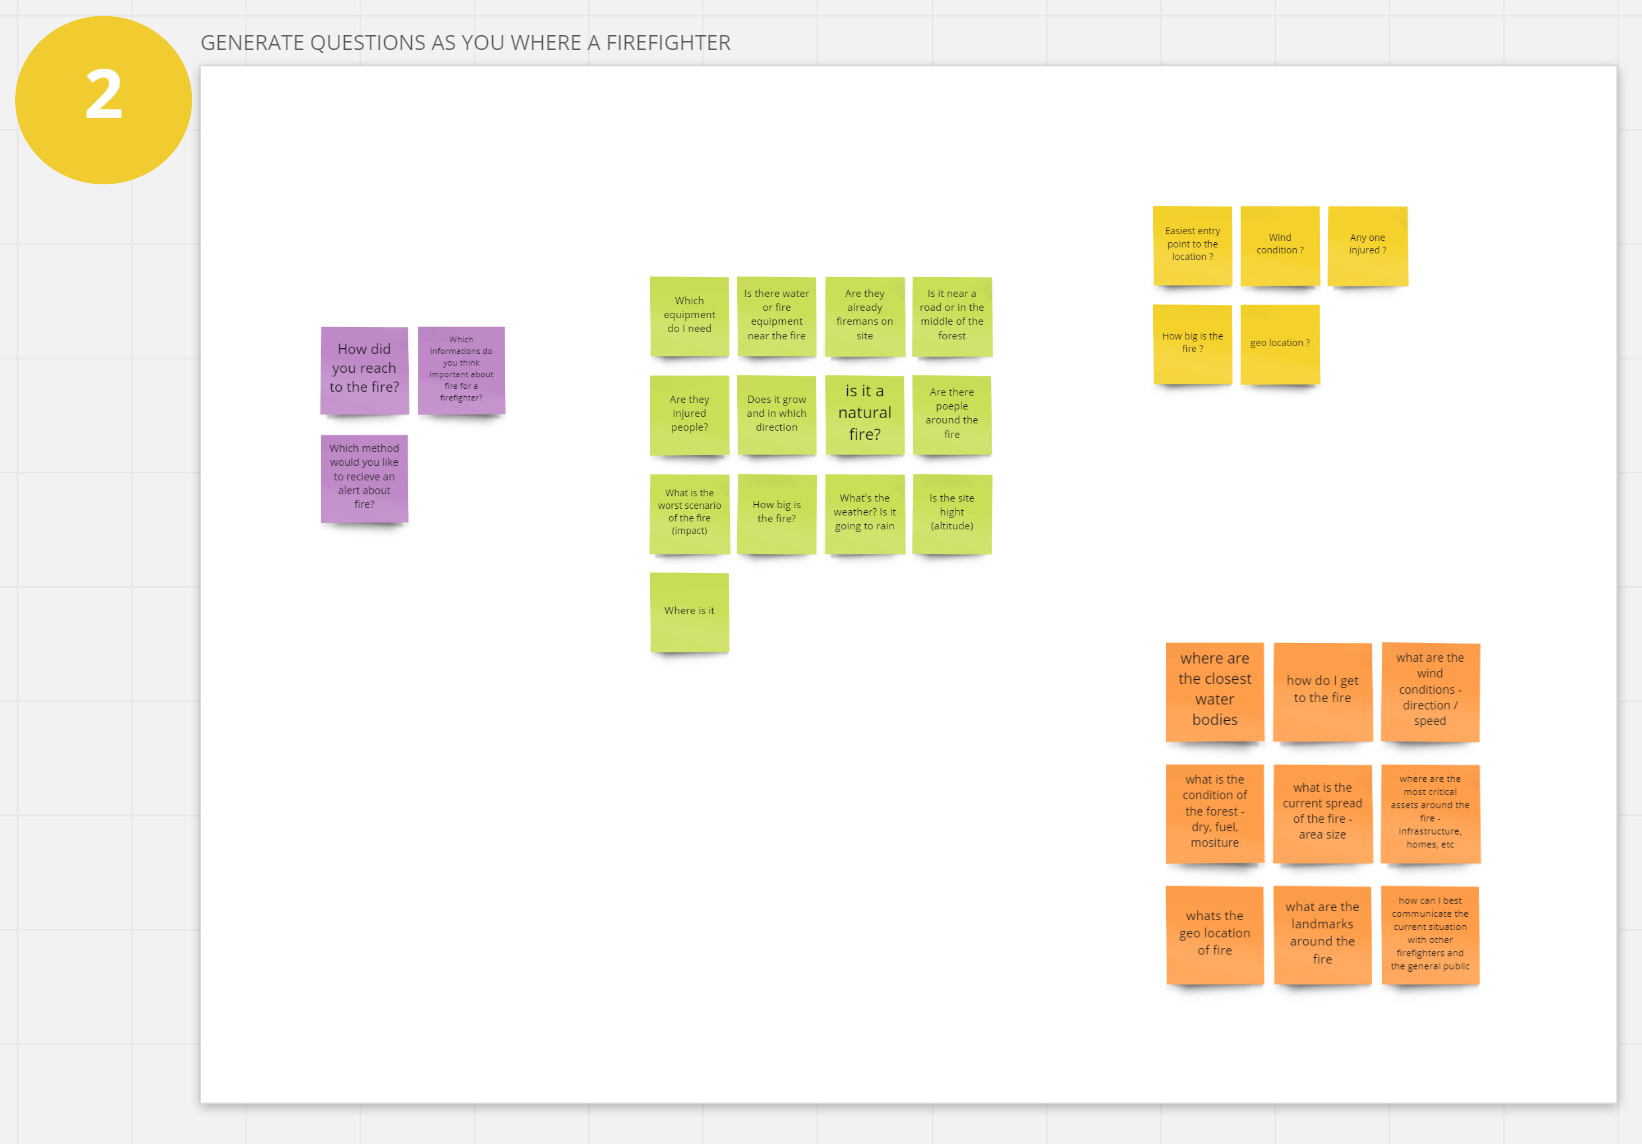
\includegraphics[width=\textwidth]{question_board_2}
  \caption{Question Board: Kollektive Generierung von Interogationen}
  \label{fig:question_board_2}
\end{figure}
\begin{figure}[H]
  \centering
  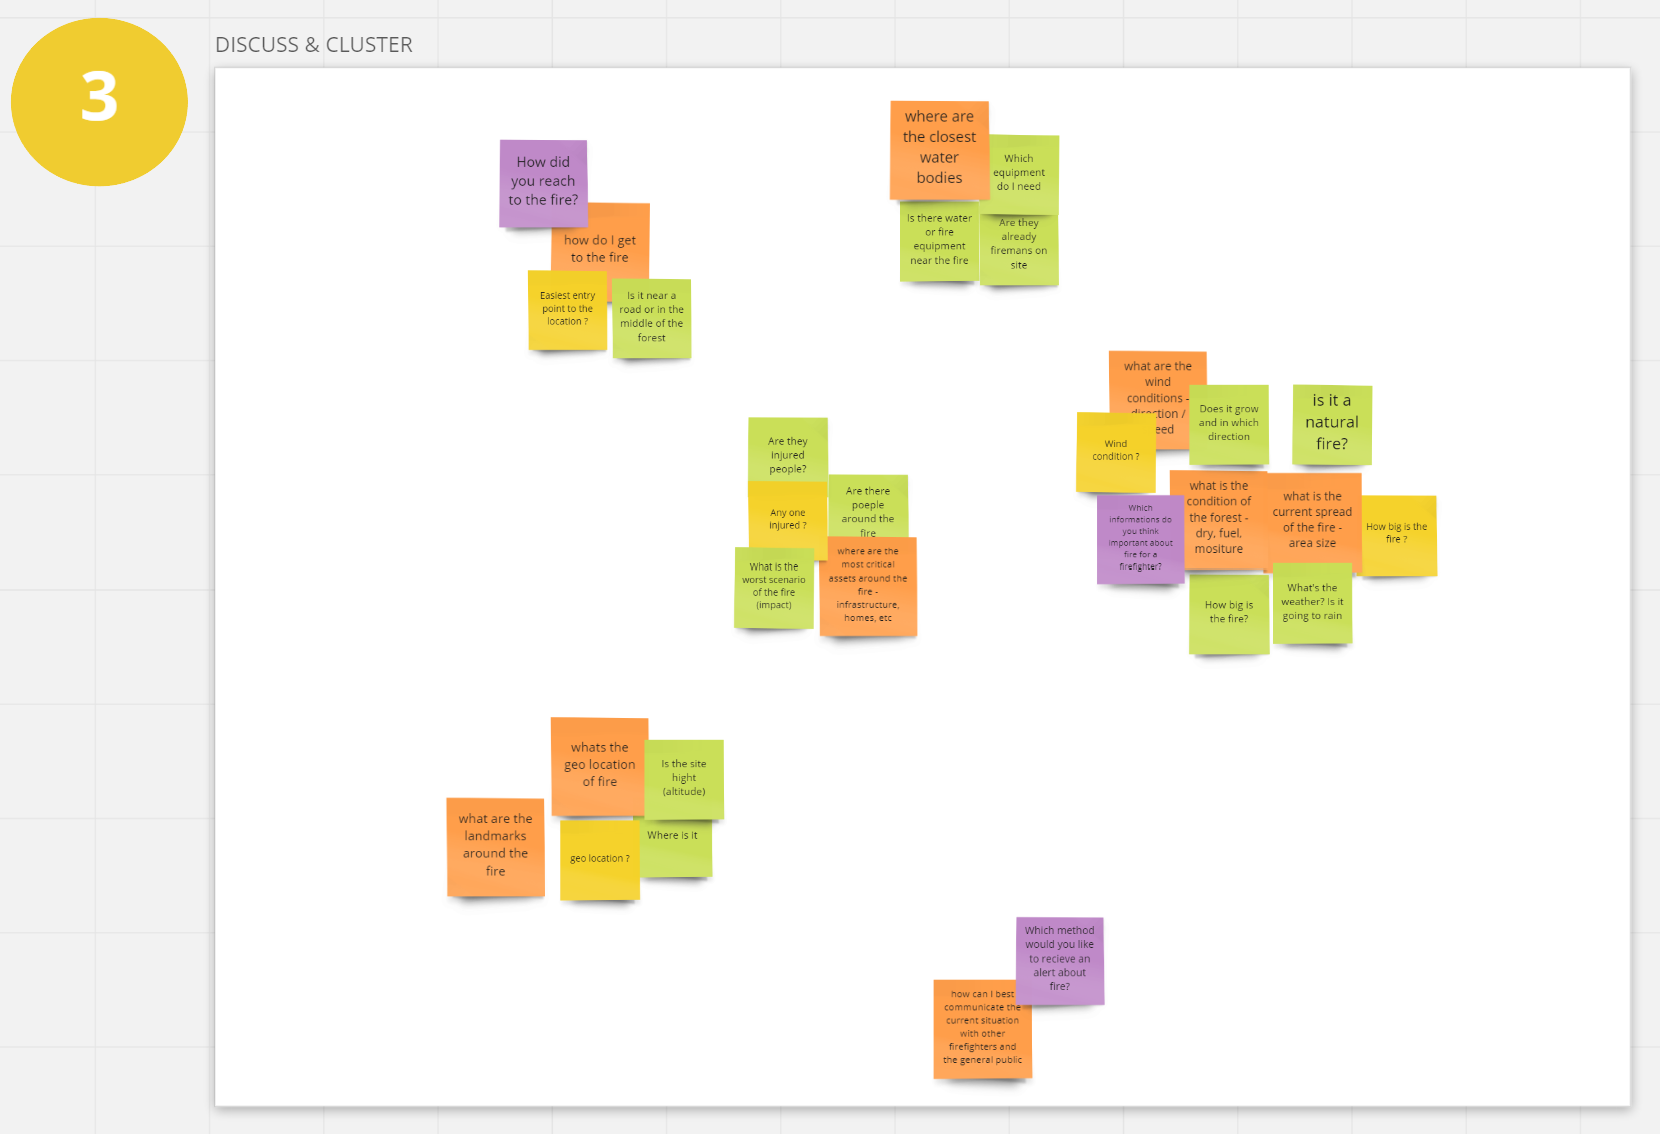
\includegraphics[width=\textwidth]{question_board_3}
  \caption{Question Board: Gruppierung von Interogationen zu gemeinsamen Themen}
  \label{fig:question_board_3}
\end{figure}
\begin{figure}[H]
  \centering
  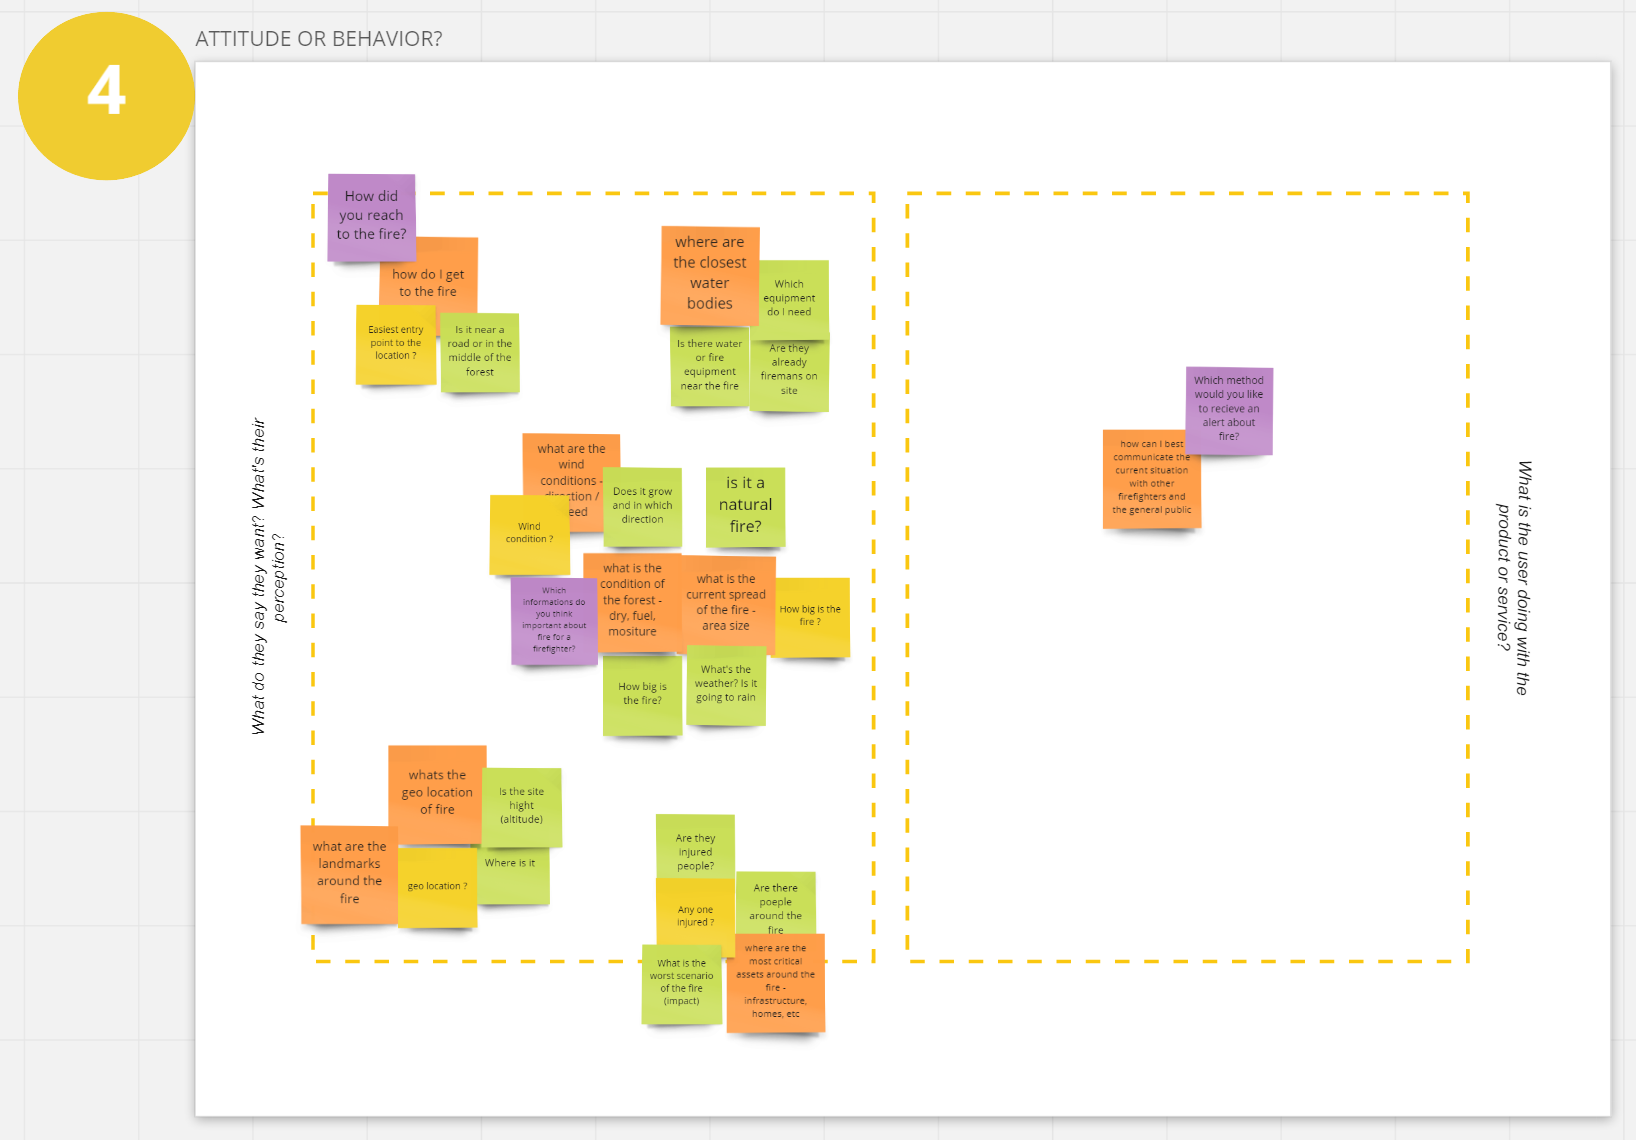
\includegraphics[width=\textwidth]{question_board_4}
  \caption{Question Board: Gruppierung der Probanden nach Interogation über Einstellung oder Verhalten}
  \label{fig:question_board_4}
\end{figure}
\begin{figure}[H]
  \centering
  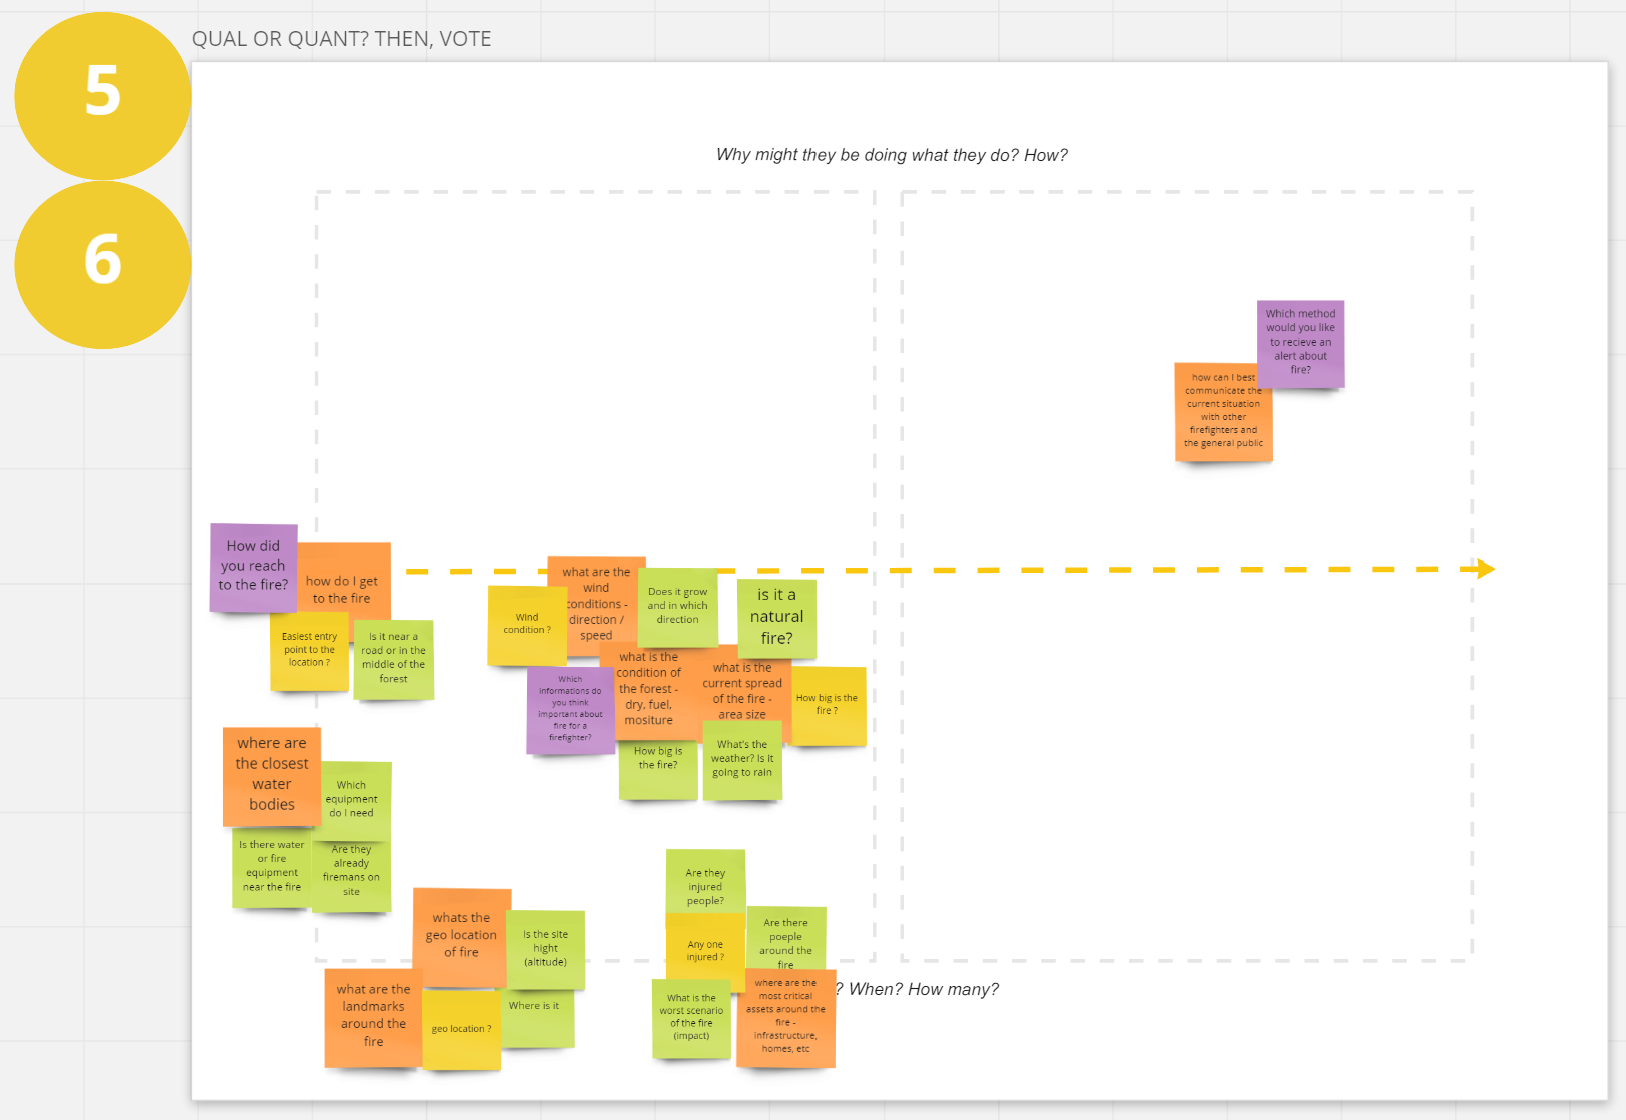
\includegraphics[width=\textwidth]{question_board_5}
  \caption{Question Board: Gruppierung der Themen nach Interogation über den quantitativen oder qualitativen Aspekt}
  \label{fig:question_board_5}
\end{figure}
\begin{figure}[H]
  \centering
  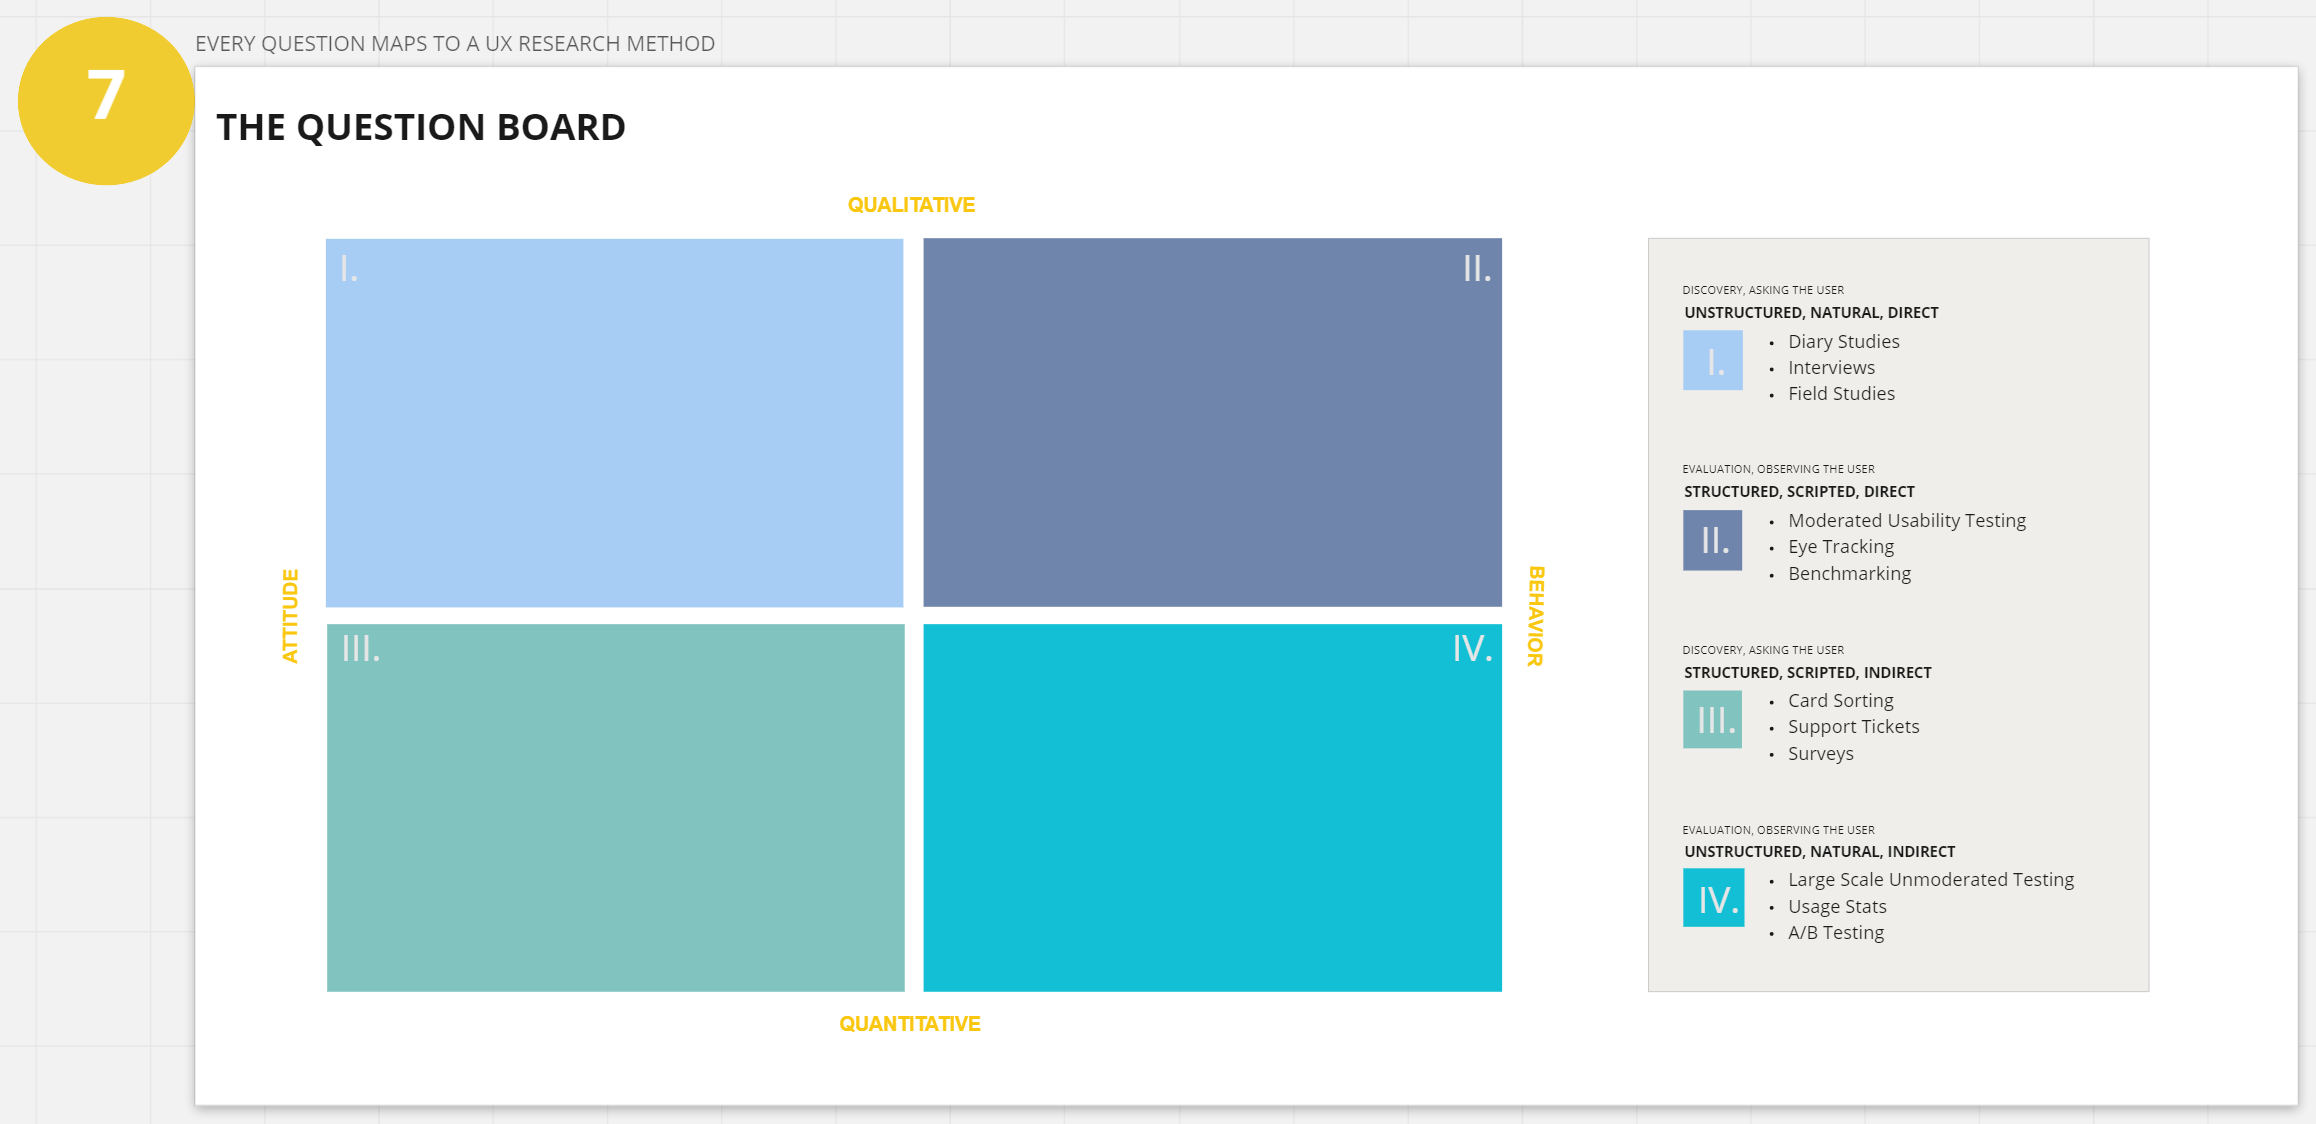
\includegraphics[width=\textwidth]{question_board_7}
  \caption{Question Board: Ansicht der möglichen Cluster mit ihrer zugehörigen Suchmethode}
  \label{fig:question_board_7}
\end{figure}